\chapter{Datastep Conversions}
\index{DataStep Conversions}
You may wonder, why would someone want to convert a datastep 
program to use tagsets?  There are lots of reasons.  Mostly it's
for code reuse and flexibility.  Datastep programs allow lots of
flexibility but they are written for one purpose.  If the same 
functionality is desired for a different set of data an entirely
new datastep will have to be written.  If the rendering is left to
a tagset, then anyone can use that tagset with any form of data,
and any procedure.  Maintenance of the code is also simplified 
since both the tagset and the resulting SAS job wil be much
simpler than the original datastep. Add the various powers of
ODS to this new found flexibility and there is plenty of motivation
for conversion.  This chapter will show the process and rewards 
of converting datastep programs to tagsets. 

\index{DDE}
\index{CSV}
\index{XML}
Yet another reason to
convert is that tagsets can be interchanged to create new and 
diffrent outputs.  Usually datastep is used to create HTML, CSV,
or DDE to XML,  A different datastep is required for each.  A different
tagset is required for each as well.  The difference is the reusability
and the ease of creation and maintenance.

\index{ODS}
\index{ODS!Styles}
\index{ODS!Select}
\index{ODS!Exclude}
\index{ODS!Document}
Full integration with ODS provides more than enough reasons to convert 
a datastep to a tagset.  Ods styles, table templates, select and exclude,
and proc document are very good reasons.  There are many other things that
ODS can do besides these, but not if datastep is the method of creating the
output.

\section{Special Bylines}
\index{nobs}
\index{Counting Observations}
\index{Bylines}
One of the things that can be done in datastep is the counting of observations
for display in the byline.  The datastep just counts them first then another
datastep prints everything out.  Tagsets can do that too.  This first example
has a special style, as well as a special byline.  The byline text may change
based upon the current by value.  Each byline also displays the number of
observations in the table below it.  

\subsection{The DataStep Code}
\index{Procedures!Report}
\index{Highlighting}
The original datastep code is shown below.  It has been simplified to use
the sashelp.class dataset.  There is nothing very hard about this code.  The
worst thing is all the puts.  The original data step also did some highlighting
and value translation.  Both of those things are much easier to do using the report procedure.
Another nice thing this datastep does is put the web page title in the title tag and
as the heading on the page.  This is also easy to do with a tagset. The original
output can be seen in figure \vref{ages_out}.

\begin{sfvcode}
filename webout 'ages.html';

%let numfuture=16;

proc sort data=sashelp.class out=myclasssrt;
  by age name weight;
run;

/* Count number of items in each BY group */
data cnt_by_obs;
   keep cnt;

   set work.myclasssrt;
   by age;

   if first.age then curcnt = 0;
   curcnt + 1;
   if last.age then do; cnt = curcnt; output; end;
run;

options missing='-';
data _null_;
   file webout;
   if _N_ = 1 then do;
      length title $ 128;
      length stoday stime $ 8;
      retain linecnt 1;

      stoday = put( today(), date7. );
      stime = put( time(), time5. ); 
      title = 'Class List &nbsp;-&nbsp; ' || stoday || "at " || stime;
      put '<!DOCTYPE HTML PUBLIC "-//IETF//DTD HTML//EN">';
      put '<HTML><HEAD>';
      put '<TITLE>' title '</TITLE>';
      put '</HEAD><BODY>';
      put '<CENTER><H3>' title '</H3></CENTER>';
   end;

   set work.myclasssrt;
   by age;

   if _N_ = 1 or FIRST.age then do;
      length lab $ 32;
      set work.cnt_by_obs;
      if age >= &numfuture then do;
         put '<CENTER><B><FONT SIZE=+2>The Oldest</FONT> ' @;
         put '<FONT SIZE=-1>(' cnt +(-1) ' '@;
         if cnt = 1 then
            put 'entry)' @;
         else
            put 'entries)' @;
         put '</FONT></B></CENTER>';
      end;
      else do;
         put '<CENTER><B><FONT SIZE=+2>Age is ' age '</FONT> ' @;
         put '<FONT SIZE=-1>(' cnt +(-1) ' '@;
         if cnt = 1 then
            put 'entry)' @;
         else
            put 'entries)' @;
         put '</FONT></B></CENTER>';
      end;
      put '<TABLE ALIGN=CENTER VALIGN=MIDDLE>';
      put '<TR>';
      lab = vlabel(Name);         put '<TH>' lab '</TH>';
      lab = vlabel(Weight);       put '<TH>' lab '</TH>';
      lab = vlabel(Height);       put '<TH>' lab '</TH>';
      lab = vlabel(Sex);          put '<TH>' lab '</TH>';
      put '</TR>';
   end;

   if mod(linecnt,2) then
      put '<TR ALIGN=CENTER VALIGN=MIDDLE BGCOLOR="D5E5D2">';
   else
      put '<TR ALIGN=CENTER VALIGN=MIDDLE>';

   put '<TD ALIGN=CENTER>' name '</TD>';
   put '<TD><FONT SIZE=-1>' weight '</FONT></TD>';
   put '<TD><FONT SIZE=-1>' height '</FONT></TD>';
   put '<TD><FONT SIZE=-1>' sex '</FONT></TD>';
   put '</TR>';

   linecnt + 1;

   if LAST.age then do;
      put '</TABLE>';
      linecnt = 1;
      put '<BR><HR><BR>';
      put '</BODY></HTML>';
   end;
run;

\end{sfvcode}

\begin{goutput}{ages_out}{Data step}
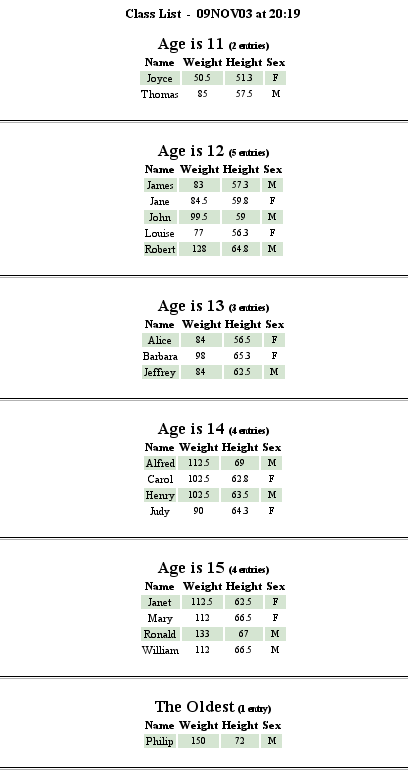
\includegraphics[width=4in]{ages.png}
\end{goutput}


\subsection{Breaking it down}
\index{Styles!Minimal}
The best way to approach a problem like this is to break it down into separate
problems.  In this case there is a fairly minimalist set of colors and fonts.
A fairly simple ODS style can be created from what can be seen in the datastep code.

\index{Tables!striping}
The next problem is striping of tables.  That problem was solved in the example on
page \pageref{striped_table}.
So this new tagset can use the stripes tagset as it's parent.  

\index{Byline!Modifying}
\index{Counting Observations}
There are three more things to solve, Extending the use of the title, counting the 
observations, and modifying the byline.  It would be perfectly
reasonable to solve both those problems in one tagset.  But the last
tagset is simpler if an
intermediate tagset is created to count the observations and display the count.
As a bonus the intermediate tagset can be used in other jobs to solve
other problems because it is not specific to this specific problem.

\subsection{The Style}
\index{Styles!Minimal}
Extracting all the colors and fonts from the datastep is easy enough.  
With something this simple the best thing is to use the minimal style as
a parent.  The minimal style will provide everything that is needed 
without making things complicated.
The resulting style looks like this.

\begin{sfvcode}
    define Style styles.minimal_striped; 
        parent = styles.minimal;

        style header/
            font = (, 4,bold)
        ;

        style Data/
            font = (, 3,normal)
        ;

        style DataStrong from data /
            background=cxD5E5D2
        ;

        replace Output /
            BorderWidth = 0
            CellSpacing = 1
            CellPadding = 7
            Frame = void
            Rules = none
        ;

    end;
\end{sfvcode}


\subsection{Counting Observations}
\index{Observation Count}
\index{Number of Observations}
\index{nobs}
\index{Variables!Macro}
The new tagset inherits from tagsets.stripes from page \pageref{striped}. 
This tagset manipulates the title and prints it as a heading. 
We also add a counter for the observations, and a stream to catch
the table while the observations are being counted.  The last thing is to add
an event to print the observation count.
A macro variable called do\_nobs\_label must be set to 'true' for the observation
counting to take effect.  Otherwise the tagset will exhibit normal behavior.
This tagset will work for any tabular output that ods creates.  
The new tagset looks like this.  
The Output is shown in listing \vref{ages2_out}.

\begin{sfvcode}
proc template;
    define tagset tagsets.nobs_label;
        parent=tagsets.stripes;

        define event initialize;
            unset $do_nobs;
            do /if $options;

                set $do_nobs "true" /if cmp($options['NOBS_LABEL']), 'yes');

                /*---------------------------------------------------eric-*/
                /*-- From the stripes tagset.                           --*/
                /*------------------------------------------------9Nov 03-*/
                set $alt_row_style $options['ALTERNATE_STYLE']";
            done;

            set $alt_row_style 'DataStrong' /if !$alt_row_style;
        end;    

        define event options_set;
            trigger initialize;
        end;

        /*-------------------------------------------------------eric-*/
        /*-- Add the date and time to the document title.  Save it  --*/
        /*-- away for later.                                        --*/
        /*----------------------------------------------------7Aug 03-*/
        define event doc_title;
              break /if ^value;
              set $title value '&nbsp;-&nbsp;' date " at " time; 
              putl '<TITLE>' $title '</TITLE>';
        end;

        define event doc_body;
            start:
                put '<body onload="startup()"';
                put ' onunload="shutdown()"';
                put  ' bgproperties="fixed"' / WATERMARK;
                putq " class=" HTMLCLASS;
                putq " background=" BACKGROUNDIMAGE;
                trigger style_inline;
                put ">" nl;
                trigger pre_post;
                put          nl;
                trigger ie_check;

                /*-----------------------------------------------eric-*/
                /*-- This is the part that changed.                 --*/
                /*-- Add in the title if we have one.               --*/
                /*--------------------------------------------7Aug 03-*/
                do /if $title;
                    putl '<h3';
                    trigger align;
                    putl '>' $title '</h3>';
                done;

            finish:
                trigger pre_post;
                put "</body>" nl;
        end;

        define event output;
            finish:
                put "<br>" nl;
        end;

        define event table ;
            start:
                eval $nobs 0;
                
                /*-----------------------------------------------eric-*/
                /*-- if we are not going to print the nobs label   --*/
                /*-- then there is no point in doing extra work.   --*/
                /*--------------------------------------------7Aug 03-*/
                open table /if cmp($do_nobs, 'true');
                set $row_class 'data';
                
                put "<div";
                trigger alt_align;
                put ">" CR;
                put '<table>' nl;
            finish:
                put '</table>' nl;
                put "</div>" nl;
                
                /*-----------------------------------------------eric-*/
                /*-- if we are not going to print the nobs label   --*/
                /*-- then there is no point in doing extra work.   --*/
                /*--------------------------------------------7Aug 03-*/
                do /if cmp($do_nobs, 'true');
                    close;
                    /* print the nobs */
                    trigger table_nobs_label; 

                    /* print the table */
                    put $$table;
                    unset $$table;
                done;
        end;
        
        /*-------------------------------------------------------eric-*/
        /*-- Count the data rows.  Swap colors.                     --*/
        /*----------------------------------------------------7Aug 03-*/
        define event row;
            start:
                /*-----------------------------------------------eric-*/
                /*-- Don not count unless we are in the data.       --*/
                /*--------------------------------------------7Aug 03-*/
                putq '<tr>' nl;
                do /if cmp(section, 'body');
                    eval $nobs $nobs+1 ;
                done;
            finish:
                put '</tr>' nl;
                /*-----------------------------------------------eric-*/
                /*-- Swap the row style at the end of the row.      --*/
                /*-- That way the first row is the one we set in    --*/
                /*-- table start.                                   --*/
                /*--------------------------------------------7Aug 03-*/
                trigger swapclass /if cmp(section, 'body');
        end;
        

        /*-------------------------------------------------------eric-*/
        /*-- Print a small heading above the table.                 --*/
        /*-- (## entries)                                           --*/
        /*----------------------------------------------------7Aug 03-*/
        define event table_nobs_label;
            style=nobs_label;
            put '<p><h4';
            putq ' class=' htmlclass; 
            put ' style="text-align: center">(' $nobs ' ';
            do /if $nobs = 1; 
                put 'entry)' ;
            else;
                put 'entries)' ;
            done;
            put '</h4></p>';
        end;
        
    end;
run;

title;


ods tagsets.nobs_label options(nobs_label='yes') 
    file="ages2.html" (title='Class List')
    style=minimal_striped;

proc sort data=sashelp.class out=myclasssrt;
    by age name sex height weight;
run;

proc print data=work.myclasssrt noobs;
    by age;
    pageby age;
run;

ods tagsets.table_nobs close;
\end{sfvcode}

\begin{goutput}{ages2_out}{Observation Counts}
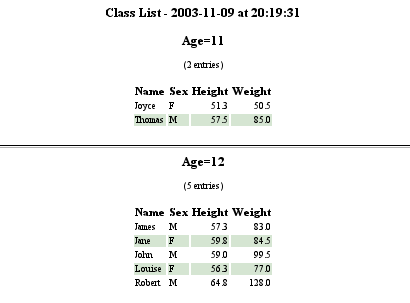
\includegraphics[width=5in]{ages2.png}
\end{goutput}

\subsection{various problems}
\index{Events!table\_head}
\index{Style!table\_head}
The first time this job runs, there is a warning in the log that the table\_head style
was not found.  This is coming from the stripes tagset where the table\_head event
is asking for the table\_head style.  It doesn't really cause any problems but defining
an empty style will take care of the warning.

\begin{sfvcode}
   style table_head
   ;
\end{sfvcode}
 
The other thing that is needed is a style for the number of observations label.  The style has
now grown to look like this.

\begin{fvcode}{datastep_style}{Refined striped style}
    define Style styles.minimal_striped; 
        parent = styles.minimal;

        style header/
            font = (, 4,bold)
        ;

        style Data/
            font = (, 3,normal)
        ;

        style DataStrong from data /
            background=cxD5E5D2
        ;

        style nobs_label from data /
        ;

        style table_head
        ;

        style byline /
           font_size = 5
           font_weight = bold
        ;

        replace Output /
            BorderWidth = 0
            CellSpacing = 1
            CellPadding = 7
            Frame = void
            Rules = none
        ;

    end;
\end{fvcode}


\subsection{Modifying the Byline}
\index{Byline!modification}
All that is left is for the byline to modified to match what the datastep code did.
This part isn't too hard either.  The easiest way to do this is to code it for the
data we are reporting on.  That makes this tagset specific to the task, and not
very reusable.  But it is a good first step.

\index{Variables!Macro}
\index{Events!Nobs\_label}
\index{Events!Byline}
Another option will work nicely to indicate which byline needs to be modified. Luckily
only one by value needs changing.  The end of the byline can be postponed until the 
table ends.  That means that the nobs event from the nobs\_count tagset can handle most 
of the work.  In the interest of versatility the byline and nobs\_label events have
been set up to work together.  If there is no byline, the nobs\_label event handles
the situation by doing the setup that the byline event would have done if there was a byline.

The new tagset and it's output follows.

\begin{fvcode}{by_age_tagset}{Tagset with modified by lines}
    define tagset tagsets.by_age;
        parent=tagsets.nobs_label;
        
        /*-------------------------------------------------------eric-*/
        /*-- Add some extra comments to the doc event.              --*/
        /*----------------------------------------------------8Aug 03-*/
        define event initialize;
            unset $do_nobs;
            do /if $options;

                do /if $options['MODIFY_BY'];
                    eval $modify_by inputn($options['MODIFY_BY'], '7.');
                    do /if missing($modify_by);
                        eval $modify_by 0;
                    done;
                done;

                set $do_nobs "true" /if cmp($options['NOBS_LABEL']), 'yes');

                /*---------------------------------------------------eric-*/
                /*-- From the stripes tagset.                           --*/
                /*------------------------------------------------9Nov 03-*/
                set $alt_row_style $options['ALTERNATE_STYLE']";
            done;

            set $alt_row_style 'DataStrong' /if !$alt_row_style;

        end;    


        /*-------------------------------------------------------eric-*/
        /*-- We want to say two different things depending on the   --*/
        /*-- value in the byline.                                   --*/
        /*----------------------------------------------------7Aug 03-*/
        define event byline;
            /*---------------------------------------------------eric-*/
            /*-- Convert age to a numeric.                          --*/
            /*------------------------------------------------7Aug 03-*/
            eval $byval inputn(scan(value, -1, '='), '7.');
        
            put '<p><div';
            putq ' class=' htmlclass ;
            put ' style="text-align: center;">' nl;

            do /if $byval = $modify_by ;
                put 'The Oldest';
            else;
                put 'Age is ' $byval ;
            done;
            
            /*---------------------------------------------------eric-*/
            /*-- A newline would do, but one way or another we need --*/
            /*-- to flush.  Otherwise the timing goes sour.         --*/
            /*------------------------------------------------8Aug 03-*/
            flush;
            set $byline "true";
        end;
        

        /*-------------------------------------------------------eric-*/
        /*-- The nobs title finishes up the paragraph started with  --*/
        /*-- the byline.                                            --*/
        /*----------------------------------------------------7Aug 03-*/
        define event table_nobs_label;
            style=nobs_label;

            /*---------------------------------------------------eric-*/
            /*-- If we did not get a byline then we want to make    --*/
            /*-- sure the html is still well formed.                --*/
            /*------------------------------------------------8Aug 03-*/
            do /if ^$byline;
                put '<p><div';
                putq ' class="byline"';
                put ' style="text-align: center">' nl;
                unset $byline;
            done;

            put '&nbsp;&nbsp;<span class="' htmlclass '">(' $nobs ' ';

            do /if $nobs = 1; 
                put 'entry)' ;
            else;
                put 'entries)' ;
            done;

            put '</span></div></p>' nl;
        end;

    end;
\end{fvcode}

The proc print that creates this output is still rather simple.  Only the two
macro variables look out of the ordinary.

\begin{sfvcode}
title;

ods tagsets.by_age options(nobs_label='yes' modify_by='16')
    file="ages3.html" (title='Class List')
    style=minimal_striped;

proc sort data=sashelp.class out=myclasssrt;
  by age name sex height weight;
run;

*options obs=6;

proc print data=work.myclasssrt noobs;
    by age;
    pageby age;
run;

ods tagsets.by_age close;
\end{sfvcode}


\begin{goutput}{ages3_out}{Output with modified By lines}
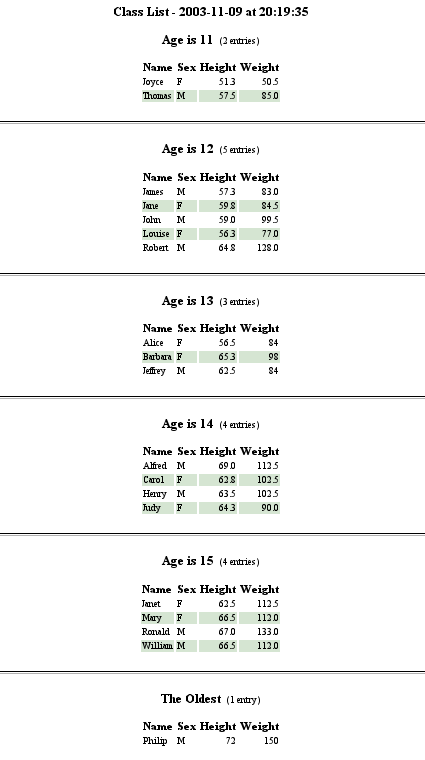
\includegraphics[width=4in]{ages3.png}
\end{goutput}

\subsection{A more flexible solution}
\index{Events!Byline}
\index{Dictionary}
This tagset is simple enough that it doesn't really matter that it's specific to this
data.  But with a little work it can be made more universal.  All it needs is a more
flexible way to indicate which by values need reformatting, and what they should be 
reformatted to.  That can be done with a macro variable. The heart of this tagset
is a dictionary.  When the proc starts the macro variable is parsed and put in 
the dictionary.  The byline event uses the dictionary to decide what to do with
each byline.  

\index{Events!Bygroup}
\subsubsection{More Identify, and Locate}
\index{ByLines}
There is an event called bygroup that surrounds all bygroup processing.  Using the start
of that event to parse the macro variable and set up the by value dictionary for the by lines
that will be coming. All of this requires that the by values are known.  But that
was a prerequesite for this particular problem anyway.

The new mod\_by\_line tagset follows.

\begin{fvcode}{flexible_byline_tagset}{A more versatile byline tagset}
 define tagset tagsets.mod_by_line;
        parent=tagsets.nobs_label;
        
        define event bygroup;
            start:
                /*-----------------------------------------------eric-*/
                /*-- Do not do this if there is no need.            --*/
                /*--------------------------------------------9Nov 03-*/
                break /if ^modify_by;

                break /if cmp($modify_by, modify_by);
                
                unset $byval_subs;
                set $modify_by modify_by;
                
                eval $count 1;
                trigger set_byval_pair;

                do /while !cmp($byval_pair, ' ');

                    set $byval_subs[$byval] $substitution;

                    eval $count $count+1;

                    trigger set_byval_pair;
                done;

        end;

        define event set_byval_pair;     
            set $byval_pair scan($modify_by, $count, '|');
            set $byval scan($byval_pair, 1, ':');
            set $substitution scan($byval_pair, 2, ':');
        end;   
        

        define event byline;
            /*---------------------------------------------------eric-*/
            /*-- Get the by value in string form                    --*/
            /*------------------------------------------------7Aug 03-*/
            eval $byval trim(scan(value, -1, '='));
            
            put '<p><div';
            putq ' class=' htmlclass ;
            put ' style="text-align: center;">' nl;

            do /if $byval_subs[$byval];
                put $byval_subs[$byval];
            else;
                do /if by_label;
                    put by_label $byval;
                else;
                    put value;
                done;
            done;
            
            /*---------------------------------------------------eric-*/
            /*-- A newline would do, but one way or another we need --*/
            /*-- to flush.  Otherwise the timing goes sour.         --*/
            /*------------------------------------------------8Aug 03-*/
            flush;
            set $byline "true";
        end;
        

        define event table_nobs_label;
            style=nobs_label;

            /*---------------------------------------------------eric-*/
            /*-- If we did not get a byline then we want to make    --*/
            /*-- sure the html is still well formed.                --*/
            /*------------------------------------------------8Aug 03-*/
            do /if ^$byline;
                put '<p><div';
                putq ' class=' htmlclass;
                put ' style="text-align: center">' nl;
                unset $byline;
            done;

            put '&nbsp;&nbsp;<span class="' htmlclass '">(' $nobs ' ';

            do /if $nobs = 1; 
                put 'entry)' ;
            else;
                put 'entries)' ;
            done;

            put '</span></div></p>' nl;
        end;

    end;
\end{fvcode}

\index{Debugging}
\index{Putlog}
\index{Statements!Putlog}
\index{Putvars}
\index{Statements!Putvars}
Tagsets like this are not all that difficult except that a mis-spelled variable or
an incorrect if statement will cause it to quietly not do what you asked.  A well placed
putlog or putvars statement can be very revealing.  In this case checking for
the options and memory variables looks like this.

\begin{sfvcode}
   putvars $options _name_ ':' _value_ ':' nl;
   putvars mem _name_ ':' _value_ ':' nl;
   putvars $byval_subs _name_ ':' _value_ ':' nl;
\end{sfvcode}

There are two things in these examples that help with debugging.  The placement
of a character on both sides of a value to reveal whitespace.  The other trick
is to separate the highly visible label from the variable by inserting another
string between them.  Then if the variable does not exist, the label will still
print.

\index{Variables!Macro}
The new job which uses the new macro variables is shown in the following job 
which creates the output in figure \ref{ages4_out} on page \pageref{ages4_out}.

\begin{sfvcode}
title;

ods tagsets.mod_by_line 
    options(nobs_label='yes' 
            by_label='Age is' 
            modify_by='16:The Oldest|11:The Youngest')
    file="ages4.html" (title='Class List')
    style=minimal_striped;

proc sort data=sashelp.class out=myclasssrt;
  by age name sex height weight;
run;

proc print data=work.myclasssrt noobs;
    by age;
    pageby age;
run;

ods tagsets.mod_by_line close;
\end{sfvcode}

\begin{goutput}{ages4_out}{Modifying Bylines, Final output}
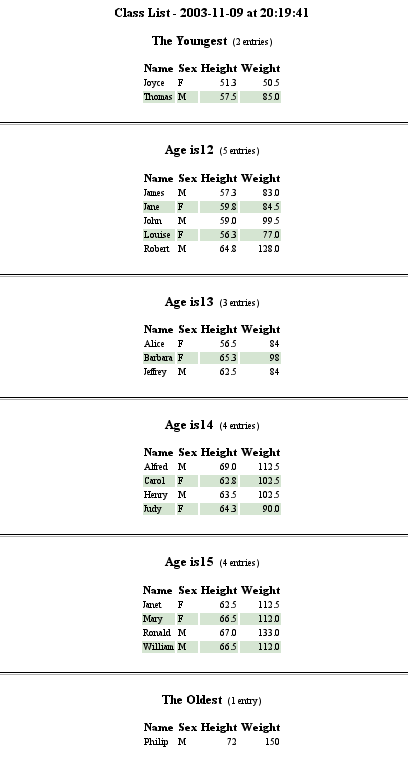
\includegraphics[width=4in]{ages4.png}
\end{goutput}


\section{Summary}
This chapter has shown some of the advantages of converting datastep code
to tagsets.  Tagsets do not pretend to replace datastep, but if responsiblities
are divided between datastep and tagsets then the solution is more open for 
re-use in later solutions.  More power and flexibility is also provided by the
tight integration the output now has with ODS.

